\section{User Requirements Definition}

La presente sezione descrive in dettaglio i requisiti utente e i casi d'uso del sistema \textbf{MyAma}, organizzati e strutturati in base alle differenti classi di attori che interagiscono con la piattaforma. Ciascuna sottosezione comprende il relativo diagramma Use Case esportato e le relative schede descrittive tabellari conformi allo standard di specifica dei requisiti.

% =========================================================================
% 3.1 UTENTE NON REGISTRATO E UTENTE DI SISTEMA
% =========================================================================
\subsection{Use Case Utente non registrato e Utente di sistema}

\subsubsection{Diagramma}
\begin{figure}[H]
    \centering
    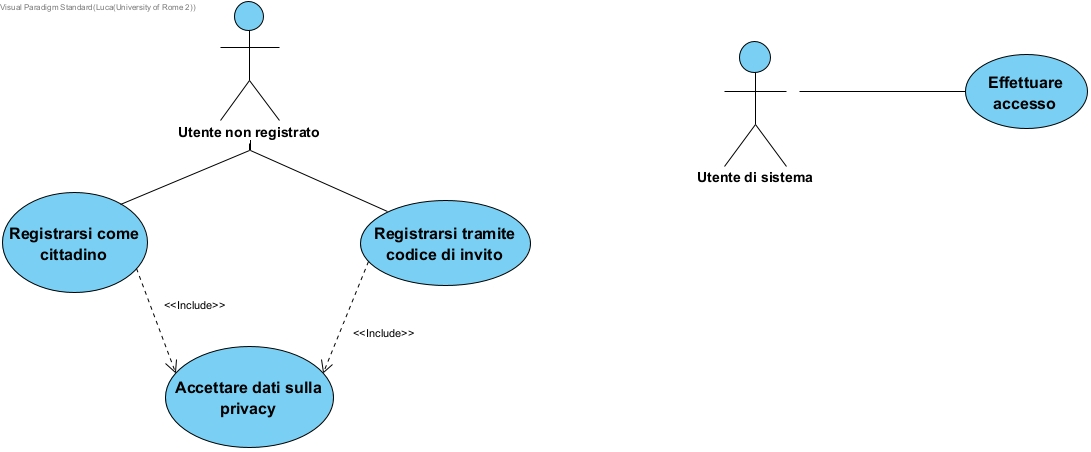
\includegraphics[width=0.75\textwidth]{figure/uc_utente_non_registrato.jpg}
    \caption{Use Case Diagram --- Utente non registrato e Utente di sistema}
    \label{fig:uc_utente_non_registrato}
\end{figure}

\subsubsection{Documentazione}

\usecasetable{Registrarsi come cittadino}{
    \textbf{Flusso delle azioni}
}{
    Utente non registrato
}{
    L'utente non possiede ancora un account nel sistema.
}{
    L'utente inserisce correttamente i dati richiesti.<br>Viene eseguito il caso d'uso "Accettare dati sulla privacy".<br>Il sistema crea l'account con il ruolo di cittadino.
}{
    L'utente inserisce dati incompleti o non validi: il sistema segnala gli errori e mostra nuovamente il form di registrazione, permettendo all'utente di correggere i dati inseriti.
}{
    L'utente risulta registrato nel sistema con il ruolo di cittadino e dispone di un account utilizzabile per accedere alle funzionalità riservate.
}

\usecasetable{Registrarsi tramite codice di invito}{
    \textbf{Flusso delle azioni}
}{
    Utente non registrato
}{
    L'utente non possiede ancora un account nel sistema e ha ricevuto un codice di invito valido.
}{
    L'utente inserisce un codice di invito valido e i dati richiesti.<br>Viene eseguito il caso d'uso "Accettare dati sulla privacy".<br>Il sistema assegna all'utente il ruolo previsto dal codice e completa la registrazione.
}{
    \begin{itemize}[leftmargin=*, nosep, topsep=2pt]
        \item Il codice di invito non è valido o è scaduto: il sistema impedisce la registrazione e segnala l'errore.
        \item I dati inseriti sono incompleti o non validi: il sistema segnala gli errori e consente all'utente di correggere i dati.
    \end{itemize}
}{
    L'utente risulta registrato nel sistema con il ruolo associato al codice di invito e dispone di un account utilizzabile per accedere alle funzionalità previste per tale ruolo.
}

\usecasetable{Accettare dati sulla privacy}{
    \textbf{Flusso delle azioni}
}{
    Utente non registrato
}{
    L'utente ha avviato una procedura di registrazione (come cittadino o tramite codice di invito) e non ha ancora completato la creazione dell'account.
}{
    Il sistema presenta l'informativa sulla privacy, l'utente la consulta e accetta il trattamento dei dati richiesto. Il sistema registra il consenso e permette di proseguire con la registrazione.
}{
    L'utente non accetta l'informativa sulla privacy: il sistema non consente di proseguire con la registrazione.
}{
    L'accettazione dell'informativa sulla privacy risulta registrata e l'utente può proseguire con la procedura di registrazione in corso.
}

\usecasetable{Effettuare accesso}{
    \textbf{Flusso delle azioni}
}{
    Utente registrato
}{
    L'utente possiede un account registrato nel sistema.
}{
    L'utente inserisce credenziali valide. Il sistema le verifica correttamente e consente l'accesso alle funzionalità associate al suo ruolo.
}{
    \begin{itemize}[leftmargin=*, nosep, topsep=2pt]
        \item Le credenziali inserite sono errate o incomplete: il sistema nega l'accesso e informa l'utente dell'errore.
        \item L'account non risulta valido o abilitato: il sistema impedisce l'accesso.
    \end{itemize}
}{
    L'utente risulta autenticato nel sistema e può utilizzare le funzionalità previste per il proprio ruolo.
}

% =========================================================================
% 3.2 CITTADINO REGISTRATO
% =========================================================================
\subsection{Use Case Cittadino registrato}

\subsubsection{Diagramma}
\begin{figure}[H]
    \centering
    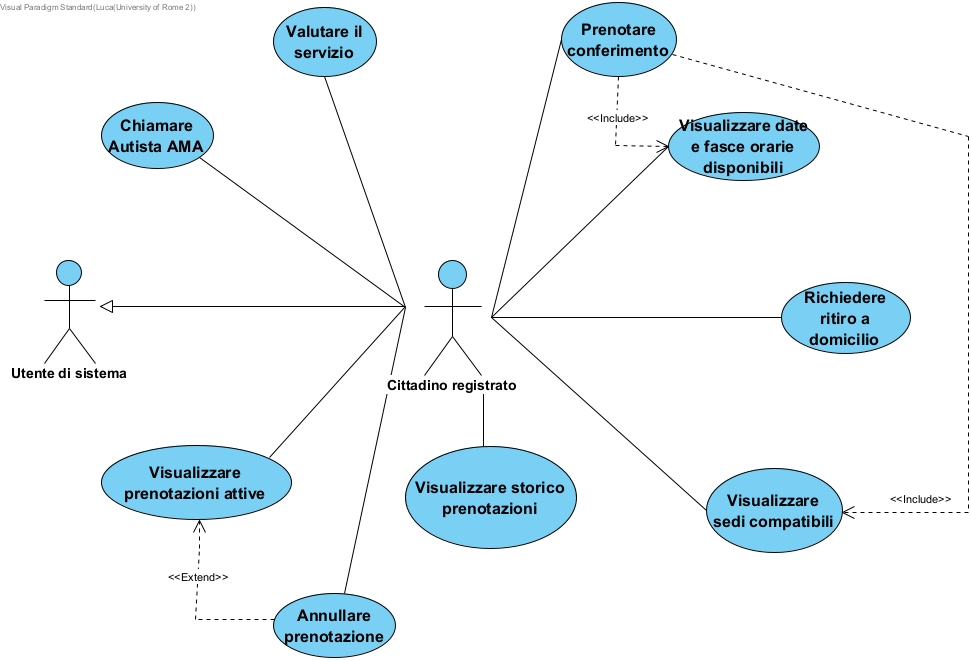
\includegraphics[width=0.85\textwidth]{figure/uc_cittadino.jpg}
    \caption{Use Case Diagram --- Cittadino registrato}
    \label{fig:uc_cittadino}
\end{figure}

\subsubsection{Documentazione}

\usecasetable{Richiedere ritiro a domicilio}{
    \textbf{Flusso delle azioni}
}{
    Cittadino registrato
}{
    Il cittadino ha effettuato l'accesso al sistema ed è abilitato all'utilizzo delle funzionalità di prenotazione.
}{
    Il cittadino inserisce correttamente le informazioni sul rifiuto e sull'indirizzo, il sistema verifica la copertura territoriale, individua una o più disponibilità e il cittadino conferma la richiesta specificando la sede compatibile e la fascia oraria. La prenotazione viene registrata.
}{
    \begin{itemize}[leftmargin=*, nosep, topsep=2pt]
        \item La zona o il CAP indicati non risultano coperti dal servizio: il sistema informa il cittadino che il ritiro non è disponibile.
        \item Non sono disponibili risorse per il ritiro: il sistema informa il cittadino dell'assenza di disponibilità.
        \item Le informazioni inserite sono incomplete o non valide: il sistema segnala gli errori e richiede al cittadino di correggere i dati.
    \end{itemize}
}{
    La richiesta di ritiro a domicilio è registrata nel sistema come prenotazione e contiene le informazioni relative al cittadino, al rifiuto, al luogo del ritiro e alla disponibilità assegnata.
}

\usecasetable{Prenotare conferimento presso sede AMA}{
    \textbf{Flusso delle azioni}
}{
    Cittadino registrato
}{
    Il cittadino ha effettuato l'accesso al sistema.
}{
    Il cittadino inserisce correttamente le informazioni e la foto del rifiuto, seleziona una sede compatibile e una disponibilità valida, e conferma il conferimento. Il sistema registra la prenotazione.
}{
    Le informazioni relative al rifiuto (o la foto caricata) sono incomplete o non valide: il sistema richiede al cittadino di correggerle prima di procedere.
}{
    La prenotazione del conferimento presso la sede AMA risulta registrata nel sistema con le informazioni relative al cittadino, al rifiuto, alla sede scelta e alla data e fascia oraria selezionate.
}

\usecasetable{Visualizzare sedi compatibili}{
    \textbf{Flusso delle azioni}
}{
    Cittadino registrato
}{
    Il cittadino ha avviato la procedura di prenotazione per il conferimento o per il ritiro, ed ha inserito le informazioni sul rifiuto.
}{
    Il sistema individua una o più sedi compatibili con la zona del cittadino e le mostra all'utente.
}{
    Non sono presenti sedi compatibili con la zona indicata: il sistema informa il cittadino che non è possibile effettuare il servizio.
}{
    Il cittadino ha selezionato una sede AMA compatibile da utilizzare per la prenotazione.
}

\usecasetable{Visualizzare date e fasce orarie disponibili}{
    \textbf{Flusso delle azioni}
}{
    Cittadino registrato
}{
    Il cittadino ha avviato la procedura di prenotazione per il conferimento o per il ritiro e ha selezionato una sede compatibile.
}{
    Il sistema individua le disponibilità compatibili con la sede scelta per il servizio richiesto (tra conferimento o ritiro) e le mostra al cittadino.
}{
    Non sono presenti date o fasce orarie disponibili per la sede selezionata: il sistema richiede di scegliere un'altra sede o di riprovare in un altro momento.
}{
    Il cittadino ha selezionato una data e una fascia oraria disponibili da utilizzare per la prenotazione.
}

\usecasetable{Annullare prenotazione}{
    \textbf{Flusso delle azioni}
}{
    Cittadino registrato
}{
    Il cittadino possiede almeno una prenotazione attiva che può essere annullata.
}{
    Il cittadino seleziona una prenotazione attiva, ne richiede l'annullamento e conferma l'operazione. Il sistema aggiorna lo stato della prenotazione.
}{
    \begin{itemize}[leftmargin=*, nosep, topsep=2pt]
        \item La prenotazione selezionata non può più essere annullata: il sistema informa il cittadino e non modifica lo stato della prenotazione.
        \item Il cittadino interrompe l'operazione prima della conferma: la prenotazione rimane invariata.
    \end{itemize}
}{
    La prenotazione risulta annullata nel sistema.
}

\usecasetable{Visualizzare prenotazioni attive}{
    \textbf{Flusso delle azioni}
}{
    Cittadino registrato
}{
    Il cittadino ha effettuato l'accesso al sistema.
}{
    Il cittadino accede all'elenco delle prenotazioni e visualizza i dettagli di quelle attive.
}{
    Il cittadino non possiede prenotazioni attive: il sistema informa che non sono presenti prenotazioni da visualizzare.
}{
    Il cittadino ha consultato l'elenco e i dettagli delle proprie prenotazioni attive.
}

\usecasetable{Visualizzare storico prenotazioni}{
    \textbf{Flusso delle azioni}
}{
    Cittadino registrato
}{
    Il cittadino ha effettuato l'accesso al sistema.
}{
    Il cittadino accede allo storico e visualizza l'elenco e i dettagli delle proprie prenotazioni passate.
}{
    Il cittadino non possiede prenotazioni concluse o annullate: il sistema informa che lo storico è vuoto.
}{
    Il cittadino ha consultato lo storico delle proprie prenotazioni (nessuna modifica allo stato del sistema).
}

\usecasetable{Valutare il servizio}{
    \textbf{Flusso delle azioni}
}{
    Cittadino registrato
}{
    Il cittadino dispone di almeno una prenotazione conclusa che può essere valutata.
}{
    Il cittadino seleziona una prenotazione conclusa, inserisce la propria valutazione e la conferma. Il sistema registra correttamente la valutazione.
}{
    Il cittadino interrompe l'operazione prima della conferma: nessuna valutazione viene registrata.
}{
    La valutazione del cittadino risulta registrata e associata alla prenotazione conclusa.
}

% =========================================================================
% 3.3 AUTISTA AMA
% =========================================================================
\subsection{Use Case Autista AMA}

\subsubsection{Diagramma}
\begin{figure}[H]
    \centering
    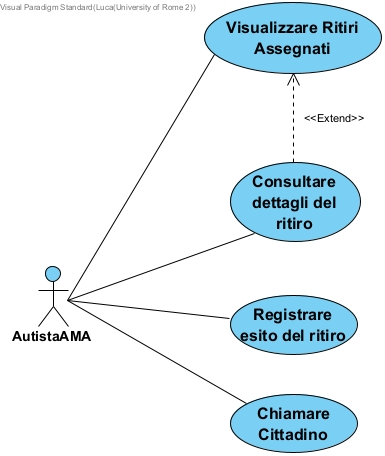
\includegraphics[width=0.85\textwidth]{figure/uc_autista.jpg}
    \caption{Use Case Diagram --- Autista AMA}
    \label{fig:uc_autista}
\end{figure}

\subsubsection{Documentazione}

\usecasetable{Visualizzare ritiri assegnati}{
    \textbf{Flusso delle azioni}
}{
    Autista AMA
}{
    L'autista AMA ha effettuato l'accesso al sistema ed è associato ad almeno un ritiro.
}{
    L'autista accede alla propria area e visualizza correttamente l'elenco dei ritiri che gli sono stati assegnati.
}{
    Non risultano ritiri assegnati all'autista: il sistema informa che non sono presenti attività da visualizzare.
}{
    L'autista ha visualizzato l'elenco dei ritiri assegnati (nessuna modifica allo stato del sistema).
}

\usecasetable{Consultare dettagli del ritiro}{
    \textbf{Flusso delle azioni}
}{
    Autista AMA
}{
    L'autista AMA ha effettuato l'accesso al sistema e ha selezionato un ritiro assegnato.
}{
    L'autista seleziona un ritiro e il sistema mostra correttamente tutte le informazioni necessarie per svolgere il servizio.
}{
    Le informazioni relative al ritiro non sono disponibili o risultano incomplete: il sistema segnala il problema all'autista.
}{
    L'autista ha consultato i dettagli del ritiro senza modificare lo stato della prenotazione.
}

\usecasetable{Registrare esito del ritiro}{
    **Flusso delle azioni
}{
    Autista
}{
    L'autista AMA ha effettuato l'accesso al sistema ed è associato al ritiro di cui deve registrare l'es
}{
    L'autista seleziona il ritiro effettuato, registra correttamente l'esito del servizio e conferma l'operazione. Il sistema aggiorna lo stato della prenotaz                                                                                                 | | \textbf{Scenari alternati L'esito inserito non è valido o è incompleto: il sistema segnala l'errore e richiede all'autista di correggere le informazioni.<br>Non è possibile aggiornare lo stato della prenotazione: il sistema segnala il problema e l'esito non viene registrato. trato. | | }Post-condizioni\textbf{     | L'esito del ritiro risulta registrato nel sistema e lo stato della prenotazione viene aggiornato di conse                                                                                                                                                  |     | }Use Case\textbf{            | }Chiamare cittadino\textbf{                                                                                                                             | | :---------------------- | :------------------------------------------------------------------------------------------------------------------------------------------------- | | }Descrizione\textbf{         | }Flusso delle azioni\textbf{                                                                                                                            | | }Attori\textbf{              | Autista AMA, Cittadino registrato                                                                                                                  | | }Precondizioni\textbf{       | L'autista AMA ha effettuato l'accesso al sistema ed è associato al ritiro relativo al cittadino da contattare.                                     | | }Scenario principale** | L'autista seleziona il ritiro, il sistema mostra il recapito telefonico e l'autista avvia la chiamata in autonomia tramite il proprio dispositivo.
}{
    Le informazioni di contatto non sono disponibili: il sistema segnala la mancanza del recapito all'autista, impedendogli di effettuare la chiamata.
}{
    L'autista ha visualizzato il contatto telefonico del cittadino e ha avuto la possibilità di avviare la chiamata.
}

% =========================================================================
% 3.4 OPERATORE DI SEDE AMA
% =========================================================================
\subsection{Use Case Operatore di sede AMA}

\subsubsection{Diagramma}
\begin{figure}[H]
    \centering
    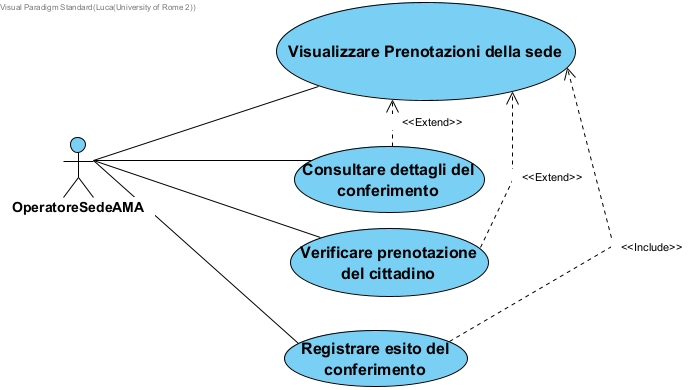
\includegraphics[width=0.85\textwidth]{figure/uc_operatore_sede.jpg}
    \caption{Use Case Diagram --- Operatore di sede AMA}
    \label{fig:uc_operatore}
\end{figure}

\subsubsection{Documentazione}

\usecasetable{Visualizzare prenotazioni della sede}{
    \textbf{Flusso delle azioni}
}{
    Operatore di sede AMA
}{
    L'operatore di sede AMA ha effettuato l'accesso al sistema ed è associato a una sede AMA.
}{
    L'operatore accede alla propria area e visualizza correttamente l'elenco delle prenotazioni associate alla sede.
}{
    Non risultano prenotazioni associate alla sede: il sistema informa l'operatore che non sono presenti conferimenti da visualizzare.
}{
    L'operatore ha visualizzato l'elenco delle prenotazioni della sede (nessuna modifica allo stato delle prenotazioni).
}

\usecasetable{Consultare dettagli del conferimento}{
    \textbf{Flusso delle azioni}
}{
    Operatore di sede AMA
}{
    L'operatore di sede AMA ha effettuato l'accesso al sistema e ha selezionato una prenotazione associata alla propria sede.
}{
    L'operatore seleziona una prenotazione e il sistema mostra correttamente tutte le informazioni necessarie relative al conferimento.
}{
    Le informazioni relative al conferimento non sono disponibili o risultano incomplete: il sistema segnala il problema all'operatore.
}{
    L'operatore ha consultato i dettagli del conferimento senza modificare lo stato della prenotazione.
}

\usecasetable{Verificare prenotazione del cittadino}{
    \textbf{Flusso delle azioni}
}{
    Operatore di sede AMA
}{
    Il cittadino possiede una prenotazione per il conferimento presso la sede AMA e si presenta per usufruire del servizio.
}{
    L'operatore individua la prenotazione del cittadino, ne verifica la validità e conferma che il conferimento possa essere effettuato.
}{
    \begin{itemize}[leftmargin=*, nosep, topsep=2pt]
        \item La prenotazione non viene trovata: il sistema informa l'operatore che non risulta alcuna prenotazione valida associata al cittadino.
        \item La prenotazione risulta annullata, non valida o riferita a una sede, data o fascia oraria diversa: il sistema segnala l'incongruenza e non consente di procedere con il conferimento.
    \end{itemize}
}{
    La prenotazione del cittadino risulta verificata e, se valida, il conferimento può essere effettuato.
}

\usecasetable{Registrare esito del conferimento}{
    \textbf{Flusso delle azioni}
}{
    Operatore di sede AMA
}{
    L'operatore di sede AMA ha effettuato l'accesso al sistema e il conferimento associato alla prenotazione è stato verificato e gestito.
}{
    L'operatore seleziona la prenotazione, registra correttamente l'esito del conferimento e conferma l'operazione. Il sistema aggiorna lo stato della prenotazione.
}{
    \begin{itemize}[leftmargin=*, nosep, topsep=2pt]
        \item L'esito inserito è incompleto o non valido: il sistema segnala l'errore e richiede all'operatore di correggere le informazioni.
        \item Non è possibile aggiornare lo stato della prenotazione: il sistema segnala il problema e l'esito non viene registrato.
    \end{itemize}
}{
    L'esito del conferimento risulta registrato nel sistema e lo stato della prenotazione viene aggiornato di conseguenza.
}

% =========================================================================
% 3.5 AMMINISTRATORE DI SEDE AMA
% =========================================================================
\subsection{Use Case Amministratore di sede AMA}

\subsubsection{Diagramma}
\begin{figure}[H]
    \centering
    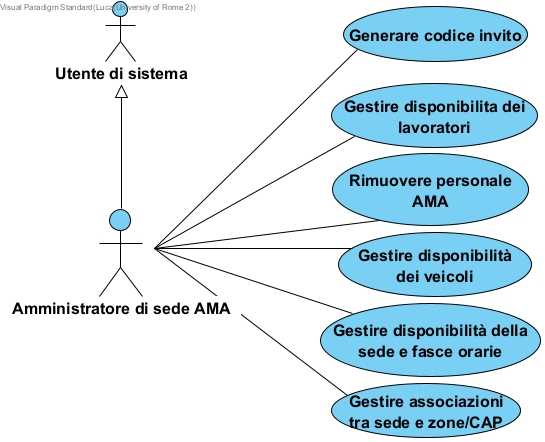
\includegraphics[width=0.85\textwidth]{figure/uc_amministratore_sede.jpg}
    \caption{Use Case Diagram --- Amministratore di sede AMA}
    \label{fig:uc_admin_sede}
\end{figure}

\subsubsection{Documentazione}

\usecasetable{Generare codice invito}{
    \textbf{Flusso delle azioni}
}{
    Amministratore di sede AMA
}{
    L'amministratore di sede AMA ha effettuato l'accesso al sistema e dispone dei permessi per generare codici invito per i ruoli di propria competenza.
}{
    L'amministratore seleziona un ruolo autorizzato e il sistema genera correttamente un codice invito utilizzabile per la registrazione del nuovo utente.
}{
    \begin{itemize}[leftmargin=*, nosep, topsep=2pt]
        \item Il ruolo selezionato non rientra tra quelli che l'amministratore di sede è autorizzato a creare: il sistema impedisce la generazione del codice.
        \item Si verifica un errore durante la generazione del codice: il sistema informa l'amministratore e non crea alcun invito valido.
    \end{itemize}
}{
    È stato generato un codice invito valido, associato al ruolo selezionato e utilizzabile da un utente non registrato per completare la relativa procedura di registrazione.
}

\usecasetable{Gestire disponibilità dei lavoratori}{
    \textbf{Flusso delle azioni}
}{
    Amministratore di sede AMA
}{
    L'amministratore ha effettuato l'accesso al sistema e il lavoratore interessato risulta associato alla sede amministrata.
}{
    L'amministratore seleziona un lavoratore, modifica correttamente le relative disponibilità e conferma l'operazione. Il sistema registra le nuove informazioni.
}{
    \begin{itemize}[leftmargin=*, nosep, topsep=2pt]
        \item Le disponibilità inserite non sono valide o risultano incomplete: il sistema segnala l'errore e richiede una correzione.
        \item Il lavoratore selezionato non risulta più associato alla sede: il sistema impedisce la modifica.
    \end{itemize}
}{
    Le disponibilità del lavoratore risultano aggiornate nel sistema e possono essere utilizzate per la pianificazione dei servizi.
}

\usecasetable{Rimuovere personale}{
    \textbf{Flusso delle azioni}
}{
    Amministratore di sede AMA
}{
    L'amministratore ha effettuato l'accesso al sistema e il membro del personale selezionato risulta associato alla sede amministrata.
}{
    L'amministratore seleziona un membro del personale, ne richiede la rimozione e conferma l'operazione. Il sistema aggiorna correttamente l'associazione.
}{
    \begin{itemize}[leftmargin=*, nosep, topsep=2pt]
        \item L'amministratore annulla l'operazione prima della conferma: nessuna modifica viene effettuata.
        \item Si verifica un errore durante la rimozione: il sistema informa l'amministratore e non modifica l'associazione.
    \end{itemize}
}{
    Il membro del personale non risulta più associato alla sede AMA amministrata.
}

\usecasetable{Gestire disponibilità dei veicoli}{
    \textbf{Flusso delle azioni}
}{
    Amministratore di sede AMA
}{
    L'amministratore ha effettuato l'accesso al sistema e il veicolo selezionato risulta associato alla sede.
}{
    L'amministratore seleziona un veicolo, modifica correttamente la sua disponibilità e conferma l'operazione.
}{
    \begin{itemize}[leftmargin=*, nosep, topsep=2pt]
        \item I dati inseriti non sono validi: il sistema segnala l'errore e richiede una correzione.
        \item Il veicolo non risulta più disponibile o associato alla sede: il sistema impedisce l'aggiornamento delle relative informazioni.
    \end{itemize}
}{
    La disponibilità del veicolo risulta aggiornata nel sistema e può essere utilizzata per la pianificazione dei ritiri.
}

\usecasetable{Gestire disponibilità della sede e fasce orarie}{
    \textbf{Flusso delle azioni}
}{
    Amministratore di sede AMA
}{
    L'amministratore ha effettuato l'accesso al sistema ed è associato alla sede da configurare.
}{
    L'amministratore modifica correttamente i giorni o le fasce orarie disponibili per i conferimenti e conferma l'operazione.
}{
    Le fasce orarie inserite non sono valide o presentano incongruenze: il sistema segnala l'errore e richiede una correzione.
}{
    Le disponibilità della sede e le relative fasce orarie risultano aggiornate e possono essere utilizzate dal sistema per le prenotazioni dei cittadini.
}

\usecasetable{Gestire associazioni tra sede e zone/CAP}{
    \textbf{Flusso delle azioni}
}{
    Amministratore di sede AMA
}{
    L'amministratore ha effettuato l'accesso al sistema ed è associato alla sede da configurare.
}{
    L'amministratore modifica correttamente le zone o i CAP associati alla propria sede e conferma l'operazione.
}{
    \begin{itemize}[leftmargin=*, nosep, topsep=2pt]
        \item La zona o il CAP indicati non sono validi: il sistema segnala l'errore e non aggiorna l'associazione.
        \item L'associazione indicata risulta già presente: il sistema informa l'amministratore e non crea un duplicato.
    \end{itemize}
}{
    Le associazioni tra la sede AMA e le relative zone o CAP risultano aggiornate e possono essere utilizzate dal sistema per determinare le sedi compatibili con le richieste dei cittadini.
}

% =========================================================================
% 3.6 AMMINISTRATORE GENERALE AMA
% =========================================================================
\subsection{Use Case Amministratore generale AMA}

\subsubsection{Diagramma}
\begin{figure}[H]
    \centering
    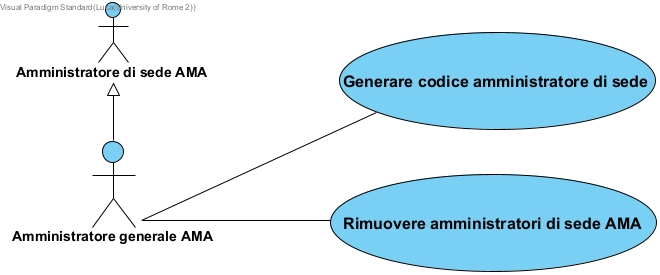
\includegraphics[width=0.75\textwidth]{figure/uc_amministratore_generale.jpg}
    \caption{Use Case Diagram --- Amministratore generale AMA}
    \label{fig:uc_admin_generale}
\end{figure}

\subsubsection{Documentazione}

\usecasetable{Generare codice amministratore di sede}{
    \textbf{Flusso delle azioni}
}{
    Amministratore generale AMA
}{
    L'amministratore generale AMA ha effettuato l'accesso al sistema e dispone dei permessi necessari per generare codici invito destinati alla registrazione di amministratori di sede AMA.
}{
    L'amministratore generale richiede la generazione di un nuovo codice invito per un amministratore di sede. Il sistema verifica i permessi, genera correttamente il codice e lo rende disponibile all'amministratore generale.
}{
    \begin{itemize}[leftmargin=*, nosep, topsep=2pt]
        \item L'amministratore generale annulla la generazione prima della conferma: nessun codice di invito viene generato.
        \item Si verifica un errore durante la generazione: il sistema informa l'amministratore generale e non produce alcun codice valido.
    \end{itemize}
}{
    È stato generato un codice invito valido associato al ruolo di amministratore di sede AMA, utilizzabile da un utente non registrato per completare la relativa procedura di registrazione.
}

\usecasetable{Rimuovere amministratori di sede AMA}{
    \textbf{Flusso delle azioni}
}{
    Amministratore generale AMA
}{
    L'amministratore generale AMA ha effettuato l'accesso al sistema e l'amministratore di sede selezionato risulta registrato e attivo nel sistema.
}{
    L'amministratore generale seleziona un amministratore di sede, ne richiede la rimozione e conferma l'operazione. Il sistema aggiorna correttamente le informazioni relative al ruolo dell'utente.
}{
    \begin{itemize}[leftmargin=*, nosep, topsep=2pt]
        \item L'amministratore generale annulla l'operazione prima della conferma: nessuna modifica viene effettuata.
        \item Si verifica un errore durante la rimozione: il sistema informa l'amministratore generale e l'utente mantiene il ruolo di amministratore di sede.
    \end{itemize}
}{
    L'utente selezionato non risulta più abilitato a operare come amministratore di sede AMA nel sistema.
}

